\documentclass[man,floatsintext]{apa6}
\usepackage{lmodern}
\usepackage{amssymb,amsmath}
\usepackage{ifxetex,ifluatex}
\usepackage{fixltx2e} % provides \textsubscript
\ifnum 0\ifxetex 1\fi\ifluatex 1\fi=0 % if pdftex
  \usepackage[T1]{fontenc}
  \usepackage[utf8]{inputenc}
\else % if luatex or xelatex
  \ifxetex
    \usepackage{mathspec}
  \else
    \usepackage{fontspec}
  \fi
  \defaultfontfeatures{Ligatures=TeX,Scale=MatchLowercase}
\fi
% use upquote if available, for straight quotes in verbatim environments
\IfFileExists{upquote.sty}{\usepackage{upquote}}{}
% use microtype if available
\IfFileExists{microtype.sty}{%
\usepackage{microtype}
\UseMicrotypeSet[protrusion]{basicmath} % disable protrusion for tt fonts
}{}
\usepackage{hyperref}
\hypersetup{unicode=true,
            pdftitle={Reproduced Report: For 5-Month-Old Infants, Melodies Are Social},
            pdfauthor={Ana Lakshin},
            pdfkeywords={music, social cognition, reproduced report, memory},
            pdfborder={0 0 0},
            breaklinks=true}
\urlstyle{same}  % don't use monospace font for urls
\usepackage{graphicx,grffile}
\makeatletter
\def\maxwidth{\ifdim\Gin@nat@width>\linewidth\linewidth\else\Gin@nat@width\fi}
\def\maxheight{\ifdim\Gin@nat@height>\textheight\textheight\else\Gin@nat@height\fi}
\makeatother
% Scale images if necessary, so that they will not overflow the page
% margins by default, and it is still possible to overwrite the defaults
% using explicit options in \includegraphics[width, height, ...]{}
\setkeys{Gin}{width=\maxwidth,height=\maxheight,keepaspectratio}
\IfFileExists{parskip.sty}{%
\usepackage{parskip}
}{% else
\setlength{\parindent}{0pt}
\setlength{\parskip}{6pt plus 2pt minus 1pt}
}
\setlength{\emergencystretch}{3em}  % prevent overfull lines
\providecommand{\tightlist}{%
  \setlength{\itemsep}{0pt}\setlength{\parskip}{0pt}}
\setcounter{secnumdepth}{0}
% Redefines (sub)paragraphs to behave more like sections
\ifx\paragraph\undefined\else
\let\oldparagraph\paragraph
\renewcommand{\paragraph}[1]{\oldparagraph{#1}\mbox{}}
\fi
\ifx\subparagraph\undefined\else
\let\oldsubparagraph\subparagraph
\renewcommand{\subparagraph}[1]{\oldsubparagraph{#1}\mbox{}}
\fi

%%% Use protect on footnotes to avoid problems with footnotes in titles
\let\rmarkdownfootnote\footnote%
\def\footnote{\protect\rmarkdownfootnote}


  \title{Reproduced Report: For 5-Month-Old Infants, Melodies Are Social}
    \author{Ana Lakshin\textsuperscript{1}}
    \date{}
  
\shorttitle{Reproduced: Melodies are Social for Infants}
\affiliation{
\vspace{0.5cm}
\textsuperscript{1} Brooklyn College}
\keywords{music, social cognition, reproduced report, memory\newline\indent Word count: X}
\usepackage{csquotes}
\usepackage{upgreek}
\captionsetup{font=singlespacing,justification=justified}

\usepackage{longtable}
\usepackage{lscape}
\usepackage{multirow}
\usepackage{tabularx}
\usepackage[flushleft]{threeparttable}
\usepackage{threeparttablex}

\newenvironment{lltable}{\begin{landscape}\begin{center}\begin{ThreePartTable}}{\end{ThreePartTable}\end{center}\end{landscape}}

\makeatletter
\newcommand\LastLTentrywidth{1em}
\newlength\longtablewidth
\setlength{\longtablewidth}{1in}
\newcommand{\getlongtablewidth}{\begingroup \ifcsname LT@\roman{LT@tables}\endcsname \global\longtablewidth=0pt \renewcommand{\LT@entry}[2]{\global\advance\longtablewidth by ##2\relax\gdef\LastLTentrywidth{##2}}\@nameuse{LT@\roman{LT@tables}} \fi \endgroup}



\authornote{Psychology Department of Brooklyn College. Psych
7709

Correspondence concerning this article should be addressed to Ana
Lakshin, 2900 Bedford Ave, Brooklyn, NY 11210. E-mail:
\href{mailto:Ana.Lakshin09@bcmail.brooklyn.cuny.edu}{\nolinkurl{Ana.Lakshin09@bcmail.brooklyn.cuny.edu}}}

\abstract{
Using Mehr et. al (2016)'s original data the following will be a
reproduction of the first experiment's analyses. The study used 5 month
old infants, two songs differing in familiarity and two unfamiliar
singers to determine if familiarity with a song will result in longer
looking times at the unfamiliar singer. It was found that infants gazed
at the unfamiliar person singing a familiar song longer than at the new
person singing an unfamiliar song.


}

\begin{document}
\maketitle

\section{Methods}\label{methods}

\subsection{Participants}\label{participants}

There were 38 full-term infants and their parents from the greater
Boston area. \#\# Procedure Parents learned to sing one of two new
songs. They sang one of the songs to their infants on a regular basis.
After 1 to 2 weeks of song exposure, the infants returned to the lab for
a selective-attention test. During the baseline trial of the test, two
unfamiliar individuals silently smiled at the infant for a brief period
of time after which each individual sang one of the two songs. After one
sang the familiar and the other sang the unfamiliar song, the two would
again silently smile and gaze at the infant.

\subsection{Data analysis}\label{data-analysis}

We used R (Version 3.5.2; R Core Team, 2019) and the R-packages
\emph{data.table} (Version 1.12.0; Dowle \& Srinivasan, 2019),
\emph{dplyr} (Version 0.8.0.1; Wickham, François, Henry, \& Müller,
2019), \emph{ggplot2} (Version 3.1.0; Wickham, 2016), \emph{ggsignif}
(Version 0.5.0; Ahlmann-Eltze, 2019), \emph{papaja} (Version 0.1.0.9842;
Aust \& Barth, 2018), \emph{pwr} (Champely, 2018), \emph{rmarkdown}
(Version 1.11; Xie, Allaire, \& Grolemund, 2018), and \emph{shiny}
(Version 1.3.0; Chang, Cheng, Allaire, Xie, \& McPherson, 2019) for all
our analyses.

\section{Results}\label{results}

In the baseline condition, there was no difference in gazes to either
singer. The mean looking time of the familiar song's singer was 52.11\%
(SD = 0.18) which was not significantly different from chance according
to the one sample T-Test \(t(31) = 0.67\), \(p = .505\).

The familiarization stage was unsuccessfully replicated. Original
results claim the duration of gazing at the singer of the familiar song
had a mean of 15.6 s with a standard deviation of 5.07. Reproduced mean
was 0.46 with standard deviation of 0.15. For duration of gazing at
singers of the unfamiliar song, the original study reported a mean of
15.3 s and standard deviation 5.10. Reproduced mean was 0.47 with
standard deviation of 0.13.

During test phase, the infants looked at the silently smiling singer of
the familiar song significantly more than chance (M= 0.59, SD = 0.18)
\(t(31) = 2.96\), \(p = .006\).

Also, during test phase the proportion of time during which the infants
gazed at the singer of the familiar song was greater than the duration
during baseline (\(t(31) = -2.42\), \(p = .022\))`.

\begin{verbatim}
## Warning in wilcox.test.default(c(0.4371257, 0.4125326, 0.754491,
## 0.4388778, : cannot compute exact p-value with ties
\end{verbatim}

\begin{figure}
\centering
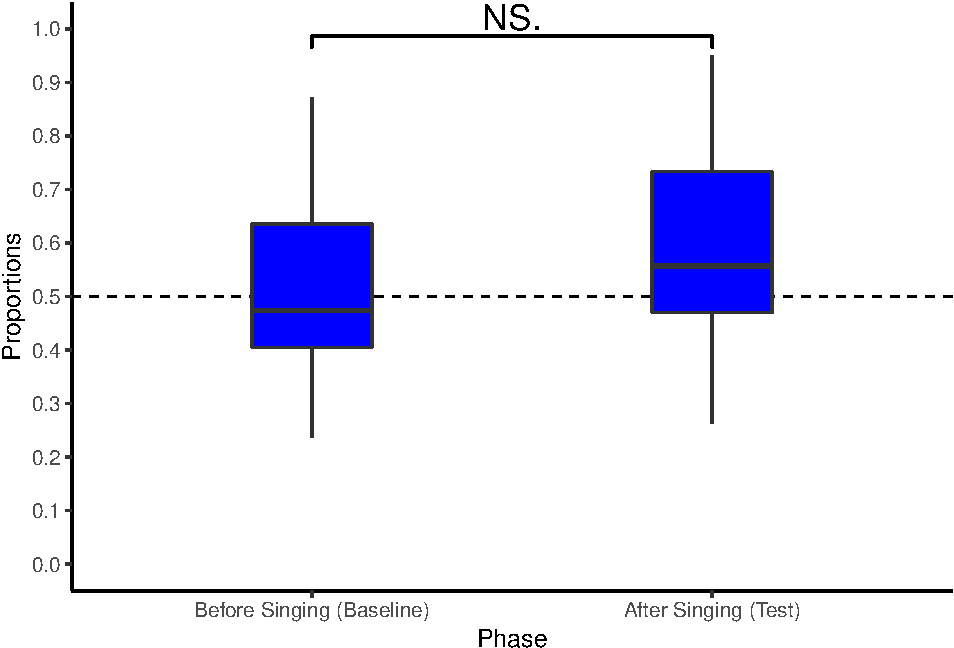
\includegraphics{Midterm_APA_files/figure-latex/unnamed-chunk-2-1.pdf}
\caption{}
\end{figure}

\begin{verbatim}
## Warning in wilcox.test.default(c(0.4371257, 0.4125326, 0.754491,
## 0.4388778, : cannot compute exact p-value with ties
\end{verbatim}

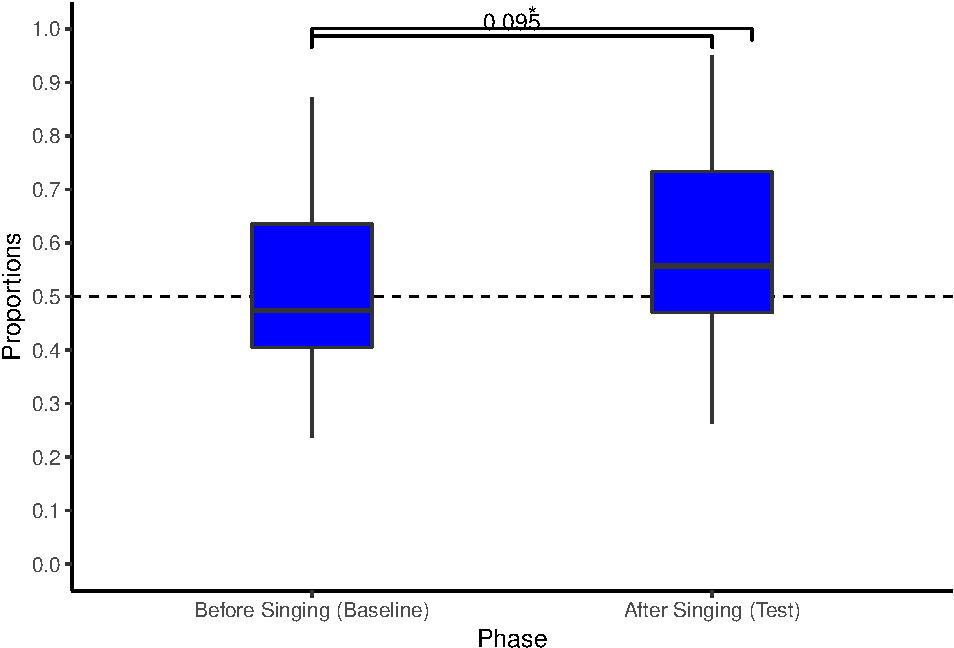
\includegraphics{Midterm_APA_files/figure-latex/unnamed-chunk-3-1.pdf}
\# Discussion Re-analysis was successful for baseline and test phase. It
was not successful for familiarization phase and for display of
significance on graph. Also, something is wrong with the bibliography
file

\subsection{Simulation-Based Power
Analysis}\label{simulation-based-power-analysis}

\begin{figure}
\centering
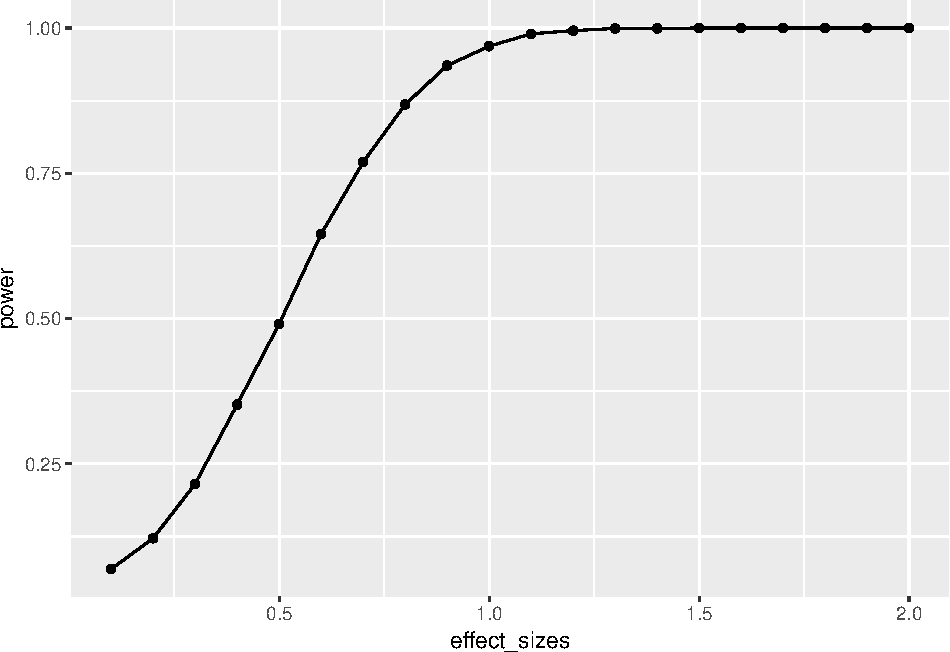
\includegraphics{Midterm_APA_files/figure-latex/unnamed-chunk-4-1.pdf}
\caption{}
\end{figure}

\newpage

\section{References}\label{references}

\begingroup
\setlength{\parindent}{-0.5in} \setlength{\leftskip}{0.5in}

\hypertarget{refs}{}
\hypertarget{ref-R-ggsignif}{}
Ahlmann-Eltze, C. (2019). \emph{Ggsignif: Significance brackets for
'ggplot2'}. Retrieved from
\url{https://CRAN.R-project.org/package=ggsignif}

\hypertarget{ref-R-papaja}{}
Aust, F., \& Barth, M. (2018). \emph{papaja: Create APA manuscripts with
R Markdown}. Retrieved from \url{https://github.com/crsh/papaja}

\hypertarget{ref-R-pwr}{}
Champely, S. (2018). \emph{Pwr: Basic functions for power analysis}.
Retrieved from \url{https://CRAN.R-project.org/package=pwr}

\hypertarget{ref-R-shiny}{}
Chang, W., Cheng, J., Allaire, J., Xie, Y., \& McPherson, J. (2019).
\emph{Shiny: Web application framework for r}. Retrieved from
\url{https://CRAN.R-project.org/package=shiny}

\hypertarget{ref-R-data.table}{}
Dowle, M., \& Srinivasan, A. (2019). \emph{Data.table: Extension of
`data.frame`}. Retrieved from
\url{https://CRAN.R-project.org/package=data.table}

\hypertarget{ref-R-base}{}
R Core Team. (2019). \emph{R: A language and environment for statistical
computing}. Vienna, Austria: R Foundation for Statistical Computing.
Retrieved from \url{https://www.R-project.org/}

\hypertarget{ref-R-ggplot2}{}
Wickham, H. (2016). \emph{Ggplot2: Elegant graphics for data analysis}.
Springer-Verlag New York. Retrieved from
\url{https://ggplot2.tidyverse.org}

\hypertarget{ref-R-dplyr}{}
Wickham, H., François, R., Henry, L., \& Müller, K. (2019). \emph{Dplyr:
A grammar of data manipulation}. Retrieved from
\url{https://CRAN.R-project.org/package=dplyr}

\hypertarget{ref-R-rmarkdown}{}
Xie, Y., Allaire, J., \& Grolemund, G. (2018). \emph{R markdown: The
definitive guide}. Boca Raton, Florida: Chapman; Hall/CRC. Retrieved
from \url{https://bookdown.org/yihui/rmarkdown}

\endgroup


\end{document}
